\PassOptionsToPackage{unicode=true}{hyperref} % options for packages loaded elsewhere
\PassOptionsToPackage{hyphens}{url}
%
\documentclass[
]{article}
\usepackage{lmodern}
\usepackage{amssymb,amsmath}
\usepackage{ifxetex,ifluatex}
\ifnum 0\ifxetex 1\fi\ifluatex 1\fi=0 % if pdftex
  \usepackage[T1]{fontenc}
  \usepackage[utf8]{inputenc}
  \usepackage{textcomp} % provides euro and other symbols
\else % if luatex or xelatex
  \usepackage{unicode-math}
  \defaultfontfeatures{Scale=MatchLowercase}
  \defaultfontfeatures[\rmfamily]{Ligatures=TeX,Scale=1}
\fi
% use upquote if available, for straight quotes in verbatim environments
\IfFileExists{upquote.sty}{\usepackage{upquote}}{}
\IfFileExists{microtype.sty}{% use microtype if available
  \usepackage[]{microtype}
  \UseMicrotypeSet[protrusion]{basicmath} % disable protrusion for tt fonts
}{}
\makeatletter
\@ifundefined{KOMAClassName}{% if non-KOMA class
  \IfFileExists{parskip.sty}{%
    \usepackage{parskip}
  }{% else
    \setlength{\parindent}{0pt}
    \setlength{\parskip}{6pt plus 2pt minus 1pt}}
}{% if KOMA class
  \KOMAoptions{parskip=half}}
\makeatother
\usepackage{xcolor}
\IfFileExists{xurl.sty}{\usepackage{xurl}}{} % add URL line breaks if available
\IfFileExists{bookmark.sty}{\usepackage{bookmark}}{\usepackage{hyperref}}
\hypersetup{
  pdftitle={Estimating the effect of luxury cabin on the chances to survive the sinking of the Titanic},
  pdfauthor={Florian Benkhalifa, Camilla Bischofberger, Max Röcker},
  pdfborder={0 0 0},
  breaklinks=true}
\urlstyle{same}  % don't use monospace font for urls
\usepackage[margin=1in]{geometry}
\usepackage{graphicx,grffile}
\makeatletter
\def\maxwidth{\ifdim\Gin@nat@width>\linewidth\linewidth\else\Gin@nat@width\fi}
\def\maxheight{\ifdim\Gin@nat@height>\textheight\textheight\else\Gin@nat@height\fi}
\makeatother
% Scale images if necessary, so that they will not overflow the page
% margins by default, and it is still possible to overwrite the defaults
% using explicit options in \includegraphics[width, height, ...]{}
\setkeys{Gin}{width=\maxwidth,height=\maxheight,keepaspectratio}
\setlength{\emergencystretch}{3em}  % prevent overfull lines
\providecommand{\tightlist}{%
  \setlength{\itemsep}{0pt}\setlength{\parskip}{0pt}}
\setcounter{secnumdepth}{-2}
% Redefines (sub)paragraphs to behave more like sections
\ifx\paragraph\undefined\else
  \let\oldparagraph\paragraph
  \renewcommand{\paragraph}[1]{\oldparagraph{#1}\mbox{}}
\fi
\ifx\subparagraph\undefined\else
  \let\oldsubparagraph\subparagraph
  \renewcommand{\subparagraph}[1]{\oldsubparagraph{#1}\mbox{}}
\fi

% set default figure placement to htbp
\makeatletter
\def\fps@figure{htbp}
\makeatother

\usepackage{dcolumn}
\usepackage{float}
\usepackage{flafter}

\title{Estimating the effect of luxury cabin on the chances to survive the
sinking of the Titanic}
\author{Florian Benkhalifa, Camilla Bischofberger, Max Röcker}
\date{3 5 2020}

\begin{document}
\maketitle

\hypertarget{introduction}{%
\subsection{Introduction}\label{introduction}}

The purpose of this paper is to assess the effect of the economic status
(class) of the cabin on the chances of survival as a passenger on the
Titanic. The fate of the R.M.S. Titanic and its passengers has captured
the attention of the whole world. There is consensus that the chances of
getting the few places in the limited number of lifeboats and surviving
the cold waters of the North Atlantic differed among social groups.
Remarkably, women rather than men survived the disaster (Hall 1986).
This was apparently due to the long time of the sinking (2.6h) that
allowed for social norms such as `women and children first' to be
established (Frey, Savage, and Torgler 2011). However, this did not
apply across cabin classes: Eyewitness reports suggest that there was a
structural disadvantage and discrimination of third-class passengers
(Diekmann 2012). Accordingly, survivors were rather from the upper cabin
classes than from lower classes (Dixon and Griffiths 2006; Frey, Savage,
and Torgler 2011; Hall 1986). Therefore, ex ante, the effect seems to be
clear -- the lower the class of a passenger, the smaller the chances for
survival. This inequality would constitute an appalling injustice and
thus, necessitates a factual verification. Fortunately, we received
passenger data from the British Board of Trade that enables us to assess
this effect. We perform a thorough analysis in the empirical framework
of a logistic regression. We find that the relationship between class
and chances of survival is best described by including additional
variables and an interaction term. We conclude that it is likely that
the effect on the survival rate might be a combination of several
factors, with economic status of the cabin being a significant one. The
results of this study should inform our struggle for safe passages for
everyone and workers rights worldwide.

\hypertarget{data-and-descriptives}{%
\subsection{Data and descriptives}\label{data-and-descriptives}}

The dataset ``Titanic'' contains information about the survival status
of a person, gender, the economic class and the age of each passenger.
All the variables are categorical, with only the economic class having
four categories - the remaining are binary.

\begin{figure}[h]

{\centering 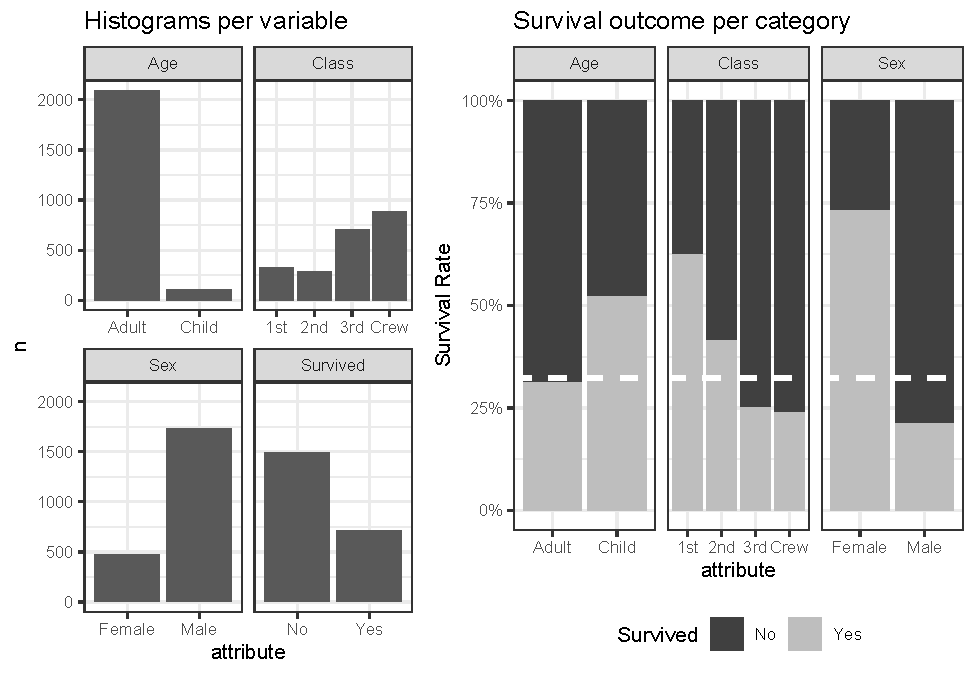
\includegraphics{Project-5_files/figure-latex/categories-1} 

}

\caption{Descriptive figures}\label{fig:categories}
\end{figure}

In total there are \(2201\) observations in the dataset. A simple
summary statistic denoting the marginal distributions of the variables
is illustrated in figure \ref{fig:categories}. In order to get a
preliminary grasp of the relation between the regressors and the target
variable, several stacked barplots are provided in Figure 1. They
graphically indicate differences in the survival rate between multiple
groups. The white dotted line marks the overall mean survivals and
facilitates to detect conspicious groups. The graph underlines three
provisional findings: - Children had a higher chance to survive than
adults, - survival rate diminishes with economic class and - females
were more likely to survive the crash than males.

From a first glance the preliminary findings seem to be linked to
traditional shipping conducts. Findings 1 and 3 mostly follow from the
``Women and children first'' policy which priorises the lives of women
and children in life threatening situations. In turn it is not
surprising that male passengers reveal a low survival rate of less than
20\%. Finding (2) would lead into the direction of the presumption about
inequality among the classes described in the introduction. Thus,
validating finding 2 is of crucial interest in the next section.

\hypertarget{empirical-strategy-and-results}{%
\subsection{Empirical strategy and
results}\label{empirical-strategy-and-results}}

In this section we estimate the causal effect of the economic status of
the cabine on the chances of survival. We start with the simplest form
of logistic regression model applicable to the data which takes the form

\[P(Survived = 1|x)= G(\beta_o + \beta_1Class1 + \beta_2Class2 + \beta_3Class3) + u\]
where \(i\) denotes the i-th individual and \(\beta_0\), \(\beta_1\),
\(\beta_2\) and \(\beta_3\) are the unknown coefficients to be
estimated. \(u\) is the error of the regression and remains unobserved.
The role of \(G\) is to keep the probability \(P(Survived = 1)\) in
between zero and one. The effect of interest is captured in equation (1)
by the beta coefficients which denote the increase of log odds when the
survival probability of survival of a passenger belonging to a lower
class is compared to a higher one. Because the coefficients are
problematic to be interpreted directly, the marginal effect,

We abstained from constructing this model via a linear relationship, as
assumed by OLS, since for some range of the covariates the estimated
conditional probability may fall outside of \([0,1]\). Clearly, such
estimations violate the premise of probability functions. Further, a
linear probability model implies that a ceteris paribus increase in
\(x_i\) always corresponds with a constant change of
\(P[Survival=1|x_i]\) regardless of the initial value of \(x_i\). This
also implies that we can get \(P[Survival=1|x_i]\) greater or less than
\([0,1]\) if we increase or decrease the dependent variable continually.
Particularly when trying to estimate partial effects for extreme values
of \(x\), this should cause concerns.

Here, the variable \(Survived\) is a binary variable indicating whether
a person survived \(Survived = 1\) or not. However, not only the
dependent variable is categorical, all explenatory are categorical as
well. To account for this specificity with regard to this paper's
purpose, namely to investigate the effect economic class on the chances
of survival, the explanatory variables are converted into three dummy
variables. This allows since the magnitude of switching from Class 1 to
Class 2, for instance, does not convey useful information, only ordinal
information.This ensures that the beta coefficients are more flexible,
since they are not bound to increase in a linear way for every class. We
have chosen to not make a dummy variable for ``Class 1'' as the effect
of being part of the first class is depicted in \(\beta_0\) while in
this case all the other ``Class'' variables are 0. Including too many
dummy to describe a group, can lead to the so-called dummy variable trap
({\textbf{???}}). Thus, the base group in this model is the first class.
Consequently, \(\beta_1\), \(\beta_2\) and \(\beta_3\) depict the
increase or decrease of the survival probabilities in comparison with
the base group. The estimation results of this simple model are
displayed in the first column of table 1.

\begin{table}[t] \centering 
  \caption{Results} 
  \label{} 
\small 
\begin{tabular}{@{\extracolsep{-24pt}}lD{.}{.}{-3} D{.}{.}{-3} D{.}{.}{-3} D{.}{.}{-3} D{.}{.}{-3} D{.}{.}{-3} D{.}{.}{-3} D{.}{.}{-3} } 
\\[-1.8ex]\hline 
\hline \\[-1.8ex] 
 & \multicolumn{8}{c}{\textit{Dependent variable:}} \\ 
\cline{2-9} 
\\[-1.8ex] & \multicolumn{8}{c}{Survived} \\ 
\\[-1.8ex] & \multicolumn{1}{c}{(1)} & \multicolumn{1}{c}{(2)} & \multicolumn{1}{c}{(3)} & \multicolumn{1}{c}{(4)} & \multicolumn{1}{c}{(5)} & \multicolumn{1}{c}{(6)} & \multicolumn{1}{c}{(7)} & \multicolumn{1}{c}{(8)}\\ 
\hline \\[-1.8ex] 
 Constant & 0.509^{***} & 2.068^{***} & 0.493^{***} & 0.500^{***} & 2.044^{***} & 2.172^{***} & 0.495^{***} & 2.182^{***} \\ 
  & (0.115) & (0.168) & (0.115) & (0.115) & (0.168) & (0.174) & (0.115) & (0.176) \\ 
  & & & & & & & & \\ 
 Class\_X2nd & -0.856^{***} & -0.953^{***} & -0.932^{***} & -0.875^{***} & -1.018^{***} & -1.037^{***} & -0.940^{***} & -1.034^{***} \\ 
  & (0.166) & (0.194) & (0.168) & (0.167) & (0.196) & (0.199) & (0.168) & (0.200) \\ 
  & & & & & & & & \\ 
 Class\_X3rd & -1.596^{***} & -1.658^{***} & -1.725^{***} & -1.641^{***} & -1.778^{***} & -1.816^{***} & -1.725^{***} & -1.810^{***} \\ 
  & (0.144) & (0.168) & (0.148) & (0.145) & (0.172) & (0.175) & (0.147) & (0.176) \\ 
  & & & & & & & & \\ 
 Class\_Crew & -1.664^{***} & -0.881^{***} & -1.648^{***} & -1.655^{***} & -0.858^{***} & -0.806^{***} & -1.650^{***} & -0.803^{***} \\ 
  & (0.139) & (0.157) & (0.139) & (0.139) & (0.157) & (0.160) & (0.139) & (0.160) \\ 
  & & & & & & & & \\ 
 Sex\_Male &  & -2.421^{***} &  &  & -2.420^{***} & -2.606^{***} &  & -2.617^{***} \\ 
  &  & (0.139) &  &  & (0.140) & (0.147) &  & (0.151) \\ 
  & & & & & & & & \\ 
 Sex\_Male\_x\_Age\_Child &  &  &  & 0.699^{***} &  & 1.795^{***} & -0.711^{*} & 1.902^{***} \\ 
  &  &  &  & (0.268) &  & (0.283) & (0.406) & (0.433) \\ 
  & & & & & & & & \\ 
 Age\_Child &  &  & 1.072^{***} &  & 1.062^{***} &  & 1.490^{***} & -0.110 \\ 
  &  &  & (0.211) &  & (0.244) &  & (0.322) & (0.335) \\ 
  & & & & & & & & \\ 
\hline \\[-1.8ex] 
cv.accuracy & 0.714 & 0.776 & 0.725 & 0.719 & 0.778 & 0.783 & 0.723 & 0.783 \\ 
cv.kap & 0.235 & 0.436 & 0.273 & 0.253 & 0.443 & 0.459 & 0.278 & 0.458 \\ 
Observations & \multicolumn{1}{c}{2,201} & \multicolumn{1}{c}{2,201} & \multicolumn{1}{c}{2,201} & \multicolumn{1}{c}{2,201} & \multicolumn{1}{c}{2,201} & \multicolumn{1}{c}{2,201} & \multicolumn{1}{c}{2,201} & \multicolumn{1}{c}{2,201} \\ 
Log Likelihood & \multicolumn{1}{c}{-1,294.278} & \multicolumn{1}{c}{-1,114.456} & \multicolumn{1}{c}{-1,281.486} & \multicolumn{1}{c}{-1,290.982} & \multicolumn{1}{c}{-1,105.031} & \multicolumn{1}{c}{-1,096.075} & \multicolumn{1}{c}{-1,279.928} & \multicolumn{1}{c}{-1,096.021} \\ 
Akaike Inf. Crit. & \multicolumn{1}{c}{2,596.555} & \multicolumn{1}{c}{2,238.913} & \multicolumn{1}{c}{2,572.972} & \multicolumn{1}{c}{2,591.965} & \multicolumn{1}{c}{2,222.061} & \multicolumn{1}{c}{2,204.150} & \multicolumn{1}{c}{2,571.855} & \multicolumn{1}{c}{2,206.043} \\ 
\hline 
\hline \\[-1.8ex] 
\textit{Note:}  & \multicolumn{8}{r}{$^{*}$p$<$0.1; $^{**}$p$<$0.05; $^{***}$p$<$0.01} \\ 
 & \multicolumn{8}{r}{Standard deviations in parentheses} \\ 
\end{tabular} 
\end{table}

The estimation results of this simple model are displayed in the first
column of table X. The Constant - b0=0.51 - is the only estimate which
is positive. Thus, this analysis suggests that the first class has the
highest chance of survival compared to the other classes and the crew.
The estimate for the crew class is the lowest with -1.66 which suggests
that being a member of the crew class has the strongest negative effect
on the chances to survive. However, the estimate for the third class is
very close to the one of the crew with -1.6. So being a passenger in the
third class or being a crew member reduces the chances of survival
almost equally compared to the first class passengers (base group). This
matches what we see in Table 1 - the survival rate of the third class
and the crew class are almost the same around 25\% and the first class
has the highest survival rate. As the estimates from our simple
regression model are all significant in the 99\% confidence bound with
p-values virtually equal to zero, we can reject the Null hypotheses that
bi=0. We now perform the model diagnostics. The important questions are
whether the estimates are credible and whether the assumptions behind
the simple model hold. In order to interpret the variable in a causal
manner, this simple randomized model works under two main assumptions:
First, that on average the error is zero \((E[u_i = 0])\) and second,
that there is randomization \((x \bot u)\) and thus, no correlation
between our error term and the Class variables (exogeneity). As we will
see further down in our analysis, these assumptions do not hold for the
simple model. The error term might contain the other variables from the
data which are gender and age. Moreover, factors contained in the error
term could be body weight, body fat, physical condition, swimming
abilities, intelligence, clothing, number of family members on the ship,
location in the ship, the distribution of flotsam and pure chance.
However, we do not have data on these factors. Our data doesn't come
from a randomized experiment but we could think of a randomized
experiment in order to extract the effect of class. We would randomly
pick 1000 people representative for all strands of society, assign them
randomly to different cabin classes on an ocean liner and let the ship
sink in the Atlantic. Fortunately, this experiment will most probably
never take place.

As we have binary variables, there is no point in adding polynomials of
higher degree to our model as this doesn't help in explaining the effect
of interest. So we are starting off by separately adding the dummy
variables for sex (column 2) and age (column 3) to the model. It is very
interesting to see how the estimates in column 2 change in comparison to
column 1. The estimates are still all significant. By adding the
variable sex (male=1), the constant which stands for the base group of
the first class, increased from 0.5 to 2.1. The estimates for the second
and third class haven't changed that much. The crew class estimate still
indicates a negative effect on the survival chance compared to the first
class. However, the estimate changed from -1.7 to -0.9. In column 2, the
estimate for being male is -2.4. To understand this, let us consider a
male first class passenger. His chance of survival would be 2.068-2.421=
-0.353. If on the other hand, we consider a female first class
passenger, her survival change would be 2.068 which is much higher as
the dummy-variable for sex is 0. The lowest survival chance would a male
third class passenger have with -2.011. Adding the age-dummy to the
simple model 1 doesn't change the estimates as much as adding a
sex-dummy as we see in column 3. The estimate for age (child=1) is also
significant and indicates a positive effect on the chances of survival.
In adding both dummy variables, we observe in column 5 the same changes
to the estimates which we observed from only adding the sex variable.
The estimates in column 5 are all significant with a very low p-value.
The change in the constant and the estimates for the classes, we can
assume that there was omitted variable bias in the simple model which
means that the above assumption of exogeneity doesn't hold. Further, we
add an interaction term to our model. There is a myriad of options for
interaction terms but we have opted to display the interaction of sex
(male=1) and age (child=1). Columns 4, 6 and 7 show the models where we
have added the interaction term separately and in combination with
either the sex dummy or the age dummy. Depending on the combination, the
estimate for the interaction term differs greatly and is least
significant and negative for model 7 where we estimate it together with
the age dummy. Column 8 depicts the estimates for the model where we
have included all the dummy variables and the interaction term. The
estimates from column 8 and column 6 are almost the same but including
all the variables decreases the bias and the chance of endogeneity in
the model.

Clearly this dataset does not deliver unbiased effects of the ecomomic
classe. In order to extract the effect of class, we could think of a
randomized experiment. Therefore, we would randomly pick 1000 people
representative for passengers who prefer to travel by a liner. For
instance, past reservations on different liners across the world could
be pooled into a dataset, and 1000 people are randomly chosen and
informed that they won a free a cruise in a lottery. Once they arrive on
the liner, which has also been randomly chosen, they are randomly
assigned to different cabin classes holding all other factors such as
ship policy equal. To eventually test how the economic class affects the
survival chance, the ship is directed towards

\begin{table}[!htbp] \centering 
  \caption{Chi-Squared for Model (1)} 
  \label{} 
\small 
\begin{tabular}{@{\extracolsep{5pt}} cccccc} 
\\[-1.8ex]\hline 
\hline \\[-1.8ex] 
 & Df & Deviance & Resid. Df & Resid. Dev & Pr(\textgreater Chi) \\ 
\hline \\[-1.8ex] 
NULL & $$ & $$ & $2,200$ & $2,769.457$ & $$ \\ 
Class\_X2nd & $1$ & $11.974$ & $2,199$ & $2,757.483$ & $0.001$ \\ 
Class\_X3rd & $1$ & $17.525$ & $2,198$ & $2,739.957$ & $0.00003$ \\ 
Class\_Crew & $1$ & $151.402$ & $2,197$ & $2,588.555$ & $0$ \\ 
\hline \\[-1.8ex] 
\end{tabular} 
\end{table}

The likelihood ratio tests indicates that adding each variable to the
regression clearly improved the model.

\begin{table}[!htbp] \centering 
  \caption{Chi-Squared for Model (8)} 
  \label{} 
\small 
\begin{tabular}{@{\extracolsep{5pt}} cccccc} 
\\[-1.8ex]\hline 
\hline \\[-1.8ex] 
 & Df & Deviance & Resid. Df & Resid. Dev & Pr(\textgreater Chi) \\ 
\hline \\[-1.8ex] 
NULL & $$ & $$ & $2,200$ & $2,769.457$ & $$ \\ 
Sex\_Male & $1$ & $434.469$ & $2,199$ & $2,334.988$ & $0$ \\ 
Age\_Child & $1$ & $5.893$ & $2,198$ & $2,329.095$ & $0.015$ \\ 
Sex\_Male\_x\_Age\_Child & $1$ & $16.319$ & $2,197$ & $2,312.776$ & $0.0001$ \\ 
Class\_X2nd & $1$ & $0.069$ & $2,196$ & $2,312.707$ & $0.793$ \\ 
Class\_X3rd & $1$ & $95.778$ & $2,195$ & $2,216.929$ & $0$ \\ 
Class\_Crew & $1$ & $24.887$ & $2,194$ & $2,192.043$ & $0.00000$ \\ 
\hline \\[-1.8ex] 
\end{tabular} 
\end{table}

The same is true for our complex model which increases over time.

\begin{table}[!htbp] \centering 
  \caption{Comparison of model (1) and (2) via a likelihood ratio test} 
  \label{} 
\small 
\begin{tabular}{@{\extracolsep{5pt}} cccccc} 
\\[-1.8ex]\hline 
\hline \\[-1.8ex] 
 & Resid. Df & Resid. Dev & Df & Deviance & Pr(\textgreater Chi) \\ 
\hline \\[-1.8ex] 
1 & $2,197$ & $2,588.555$ & $$ & $$ & $$ \\ 
2 & $2,194$ & $2,192.043$ & $3$ & $396.513$ & $0$ \\ 
\hline \\[-1.8ex] 
\end{tabular} 
\end{table}

We finally make a likelihood ratio test to find out if the complex model
really outperforms the simple model. The p-value is significant
indicating that the complex model increased the performance.

\hypertarget{conclusion}{%
\subsection{Conclusion}\label{conclusion}}

In summary, the economic status of the cabin (class) appears to have an
effect on the survival chances. The positive effect which a passenger in
the first class enjoys on its survival chances decreases with economic
class (crew included). Thus, our findings concur with the literature. In
consequence, we suggest a policy change that makes the Atlantic passage
safe for all passengers, regardless of class. This could include raising
the number of lifeboats and life vests to a number that reflects the
passenger numbers and ensuring that lifeboats can easily be accessed
from different cabin class areas.

\hypertarget{references}{%
\section{References}\label{references}}

\hypertarget{refs}{}
\leavevmode\hypertarget{ref-diekmann2012}{}%
Diekmann, Andreas. 2012. ``Die Rolle sozialer Normen, der
Situationsdefinition und sozialer Klassen beim Untergang der Titanic.''
\emph{KZfSS Kölner Zeitschrift Für Soziologie Und Sozialpsychologie} 64
(1): 175--84. \url{https://doi.org/10.1007/s11577-012-0160-y}.

\leavevmode\hypertarget{ref-dixon2006}{}%
Dixon, Robert, and William Griffiths. 2006. ``Survival on the Titanic:
Illustrating Wald and Lagrange Multiplier Tests for Proportions and
Logits.'' \emph{The Journal of Economic Education} 37 (3): 289--304.
\url{https://doi.org/10.3200/JECE.37.3.289-304}.

\leavevmode\hypertarget{ref-frey2011}{}%
Frey, Bruno S, David A Savage, and Benno Torgler. 2011. ``Behavior Under
Extreme Conditions: The \emph{Titanic} Disaster.'' \emph{Journal of
Economic Perspectives} 25 (1): 209--22.
\url{https://doi.org/10.1257/jep.25.1.209}.

\leavevmode\hypertarget{ref-hall1986}{}%
Hall, Wayne. 1986. ``Social Class and Survival on the S.S. Titanic.''
\emph{Social Science \& Medicine} 22 (6): 687--90.
\url{https://doi.org/10.1016/0277-9536(86)90041-9}.

\end{document}
